% Options for packages loaded elsewhere
\PassOptionsToPackage{unicode}{hyperref}
\PassOptionsToPackage{hyphens}{url}
%
\documentclass[ignorenonframetext, ]{beamer}
% \usepackage{showframe}
% ---------------------------------------------------------------%
\usetheme[]{Copenhagen}
\useoutertheme{infolines}
\setbeamertemplate{navigation symbols}{}
\usepackage{subcaption}
\usepackage{graphicx}
\usepackage{pgfpages}
% Prevent slide breaks in the middle of a paragraph
\usepackage{amsmath,amssymb}
% Use upquote if available, for straight quotes in verbatim environments
\IfFileExists{upquote.sty}{\usepackage{upquote}}{}
\providecommand{\tightlist}{%
  \setlength{\itemsep}{0pt}\setlength{\parskip}{0pt}}
\setcounter{secnumdepth}{-\maxdimen} % remove section numbering
\usepackage{tikz-cd}
\usepackage{adjustbox}
\title{Was Rasmus Nielsen a Windbag?}
\author{Hans Halvorson}
\date{November 24, 2023}

\begin{document}
\frame{\titlepage}

\section{Introduction}

\begin{frame}

  \begin{tabular}{cc}
            \parbox[b]{0.5\linewidth}{ %  change the parbox width as
            % appropiate
      Rasmus Nielsen was a 19th century philosopher from Copenhagen
      whose work has been utterly forgotten.
      } 
      &          \begin{tabular}{c}
                   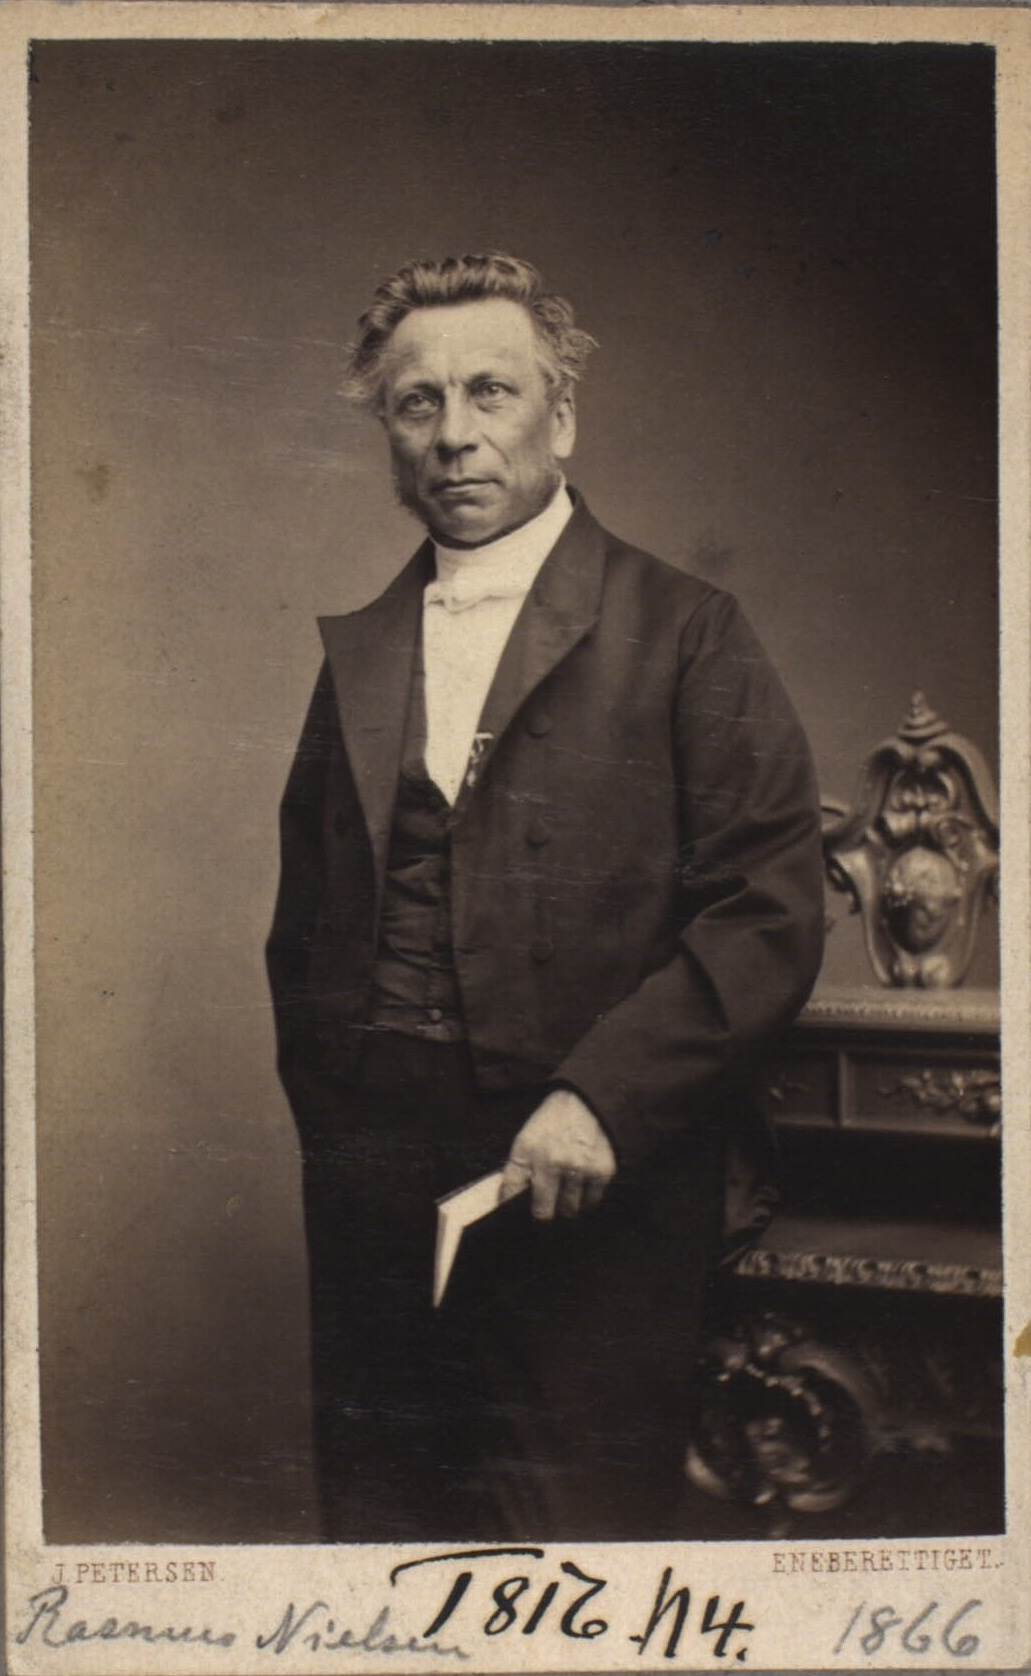
\includegraphics[scale=0.45]{nielsen-small.jpg} \\
                   {\small Rasmus Nielsen } \\
                   {\small (1809--1884) }
           \end{tabular}  \\
  \end{tabular}

  %% TO DO: I would like to figure out how to have the text on the
  %% left come out on the top

\end{frame}

\begin{frame}{Introduction}
  
  \begin{itemize}
  \item If you've heard of Nielsen, that's probably because he's
    discussed briefly in Garff's biography. SK originally thought of
    Nielsen as his comrade in arms, but then pushed him away.
  \item Not a single page of the thousands that Nielsen wrote has been
    translated to a ``world language''.
  \item I will begin by explaining reasons to be interested in Nielsen
    --- not just for historians, but also for understanding our
    contemporary predicament.
\end{itemize}

\end{frame}

\begin{frame}{Four reasons to be interested in Nielsen}

\begin{enumerate}
\item Kierkegaard
\item Niels Bohr
\item Nielsen upsets standard narratives about the novelty of analytic
  philosophy.
\item Nielsen develops a Kierkegaard-inspired philosophy of science
  --- and so provides a link between Kierkegaard and science.
\end{enumerate}

\end{frame}

\begin{frame}{1. Kierkegaard}
  
\begin{itemize}
\item Nielsen's relevance for Kierkegaard studies is described well in
  Jon Stewart, ``Rasmus Nielsen: From the object of `prodigious
  concern' to a `windbag'\,''.
\item Nielsen deserves the credit for transmitting SK's ideas to
  subsequent generations (Brandes, Høffding, etc.).
\item Nielsen is ``patient zero'' for reception and transformation of
  SK's ideas.
\end{itemize}  
\end{frame}


\begin{frame}{2. Bohr}
  \begin{itemize}
\item My project began with wanting to make sense, philosophically, of
  contemporary physics. What do all of these new discoveries mean for
  us?
\item Niels Bohr had wrestled with such questions more than anyone
  else.
\item But contemporary philosophers are either uninterested in Bohr,
  or say that they cannot make sense of him, or say that he was
  obviously wrong.
\item Bohr did have one defender \dots 
\end{itemize}
\end{frame}

\begin{frame}

\begin{figure}
\centering
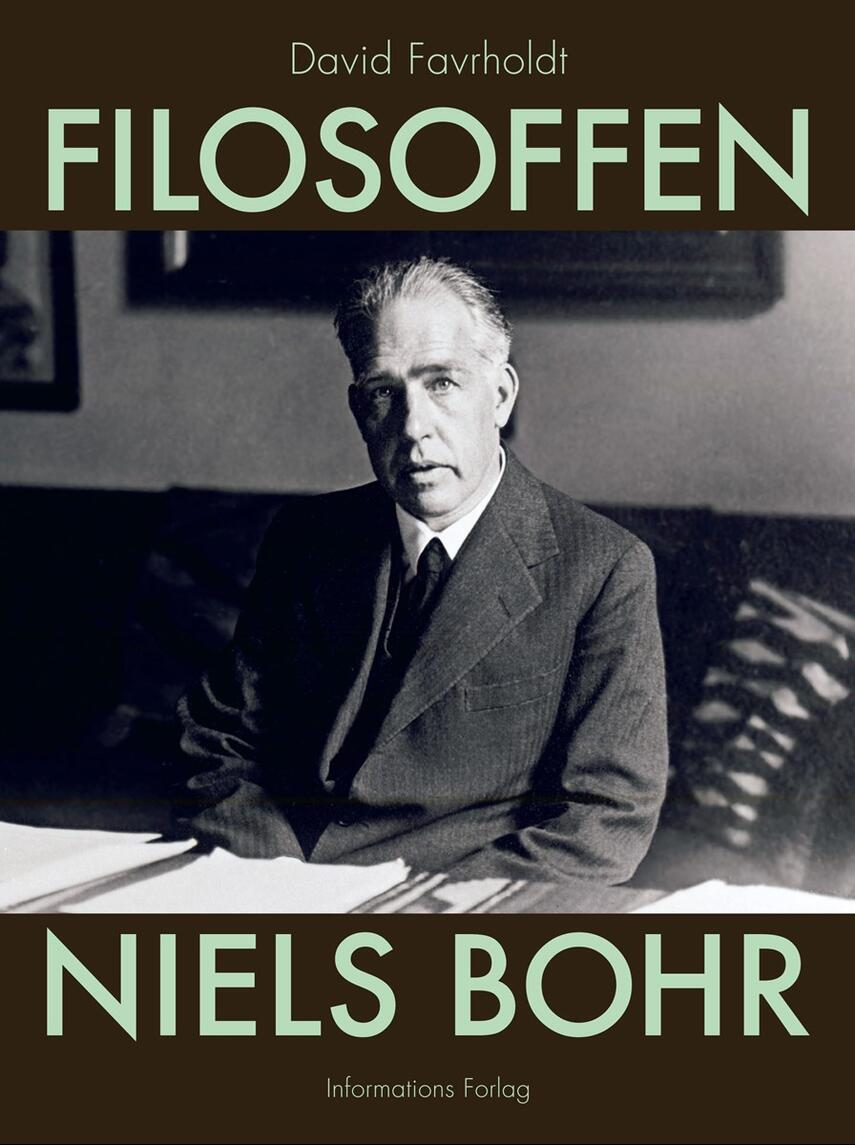
\includegraphics[scale=0.28]{filosoffen.jpg}
\end{figure}
\end{frame}

\begin{frame}{Favrholdt makes explicit what Bohr left implicit}

\begin{figure}
  \centering 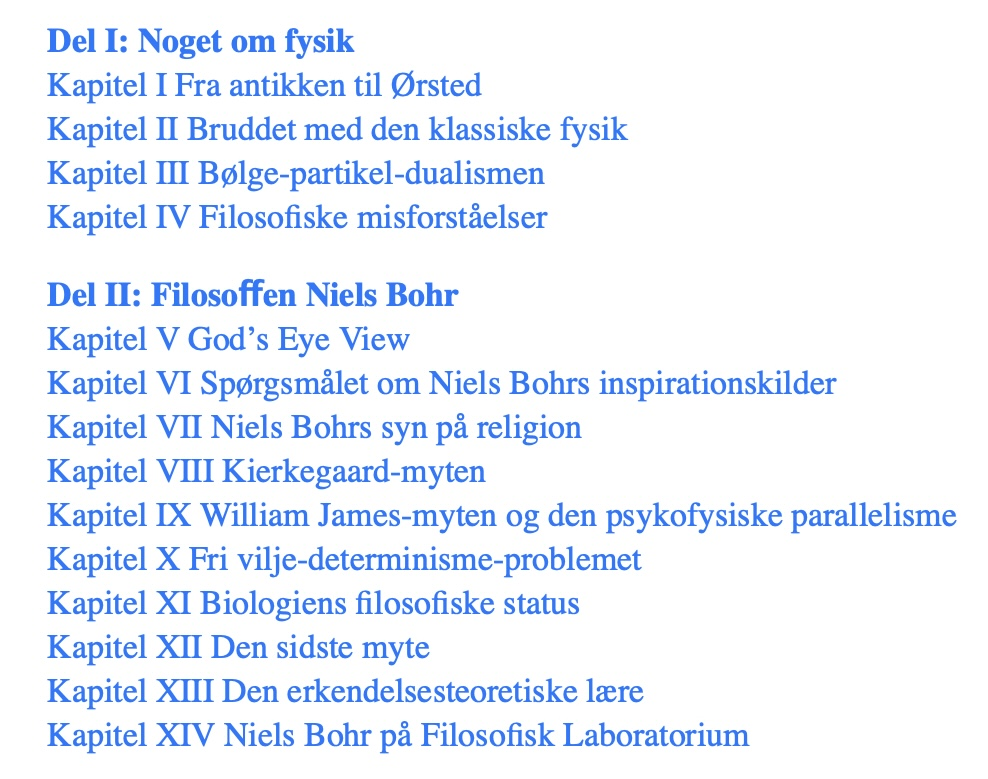
\includegraphics[scale=0.5]{indhold.jpg}
\end{figure}
\end{frame}

\begin{frame}

\begin{itemize}
\item Contemporary philosophers write Bohr off as being a logical
  positivist, or unclear, or [fill in the blank].
\item Others argue that he is Kantian.
\item Denmark has its own philosophical tradition that doesn't fit
  neatly into this ``world historic'' classification scheme.
\item One is struck by thematic similarities between Bohr's philosophy
  and Kierkegaard's (especially \emph{Postscript}).
  \begin{itemize}
  \item Favrholdt unequivocally denies that Bohr was influenced by
    Kierkegaard.
  \end{itemize}
\end{itemize}
\end{frame}

\begin{frame}

  \textbf{Hypothesis:} Nielsen transformed Kierkegaard's
  epistemological ideas into something that was accessible to
  scientifically minded people such as Bohr.

  \vspace{2em}

\adjustbox{scale=0.8,center}{%
\begin{tikzcd}[ampersand replacement = \&]
  \&\&\&\& \text{H. Høffding} \\
  \text{S. Kierkegaard} \&\& \text{R. Nielsen} \&\&\&\& \text{N. Bohr} \\
  \&\&\&\& \text{Ch. Bohr} \arrow[from=2-1, to=2-3] \arrow[from=2-3,
  to=1-5] \arrow[from=2-3, to=3-5] \arrow[from=1-5, to=2-7]
  \arrow[from=3-5, to=2-7]
\end{tikzcd}
}

\end{frame}

\begin{frame}{3. Nielsen challenges the dominant narrative}

\begin{itemize}
\item At a given moment in history, philosophers from prevailing
  cultures tend to see the history of philosophy as leading up to
  them.
  \begin{itemize}
  \item Hegel
  \item Reichenbach. \emph{The Rise of Scientific Philosophy}
  \item Anglo-american philosophy
  \end{itemize}
\item Example: The apriori from Kant to Carnap to Quine
\end{itemize}

\end{frame}

\begin{frame}{3. Nielsen challenges the dominant narrative}

\begin{itemize}
\item Nielsen's philosophy has several themes in common with Marburg
  neo-kantianism (especially Cassirer and Reichenbach).
  \begin{itemize}
  \item Nielsen claims that science always has apriori truths, but
    they are changeable.
  \end{itemize}
\item Nielsen's view of the relationship between philosophy and
  science anticipates themes in logical positivism and in contemporary
  philosophy of science.
\end{itemize}
\end{frame}

\begin{frame}{4. Nielsen links Kierkegaard to science}

  As for Nielsen providing a bridge between Kierkegaard and science,
  that will emerge in what follows!


\end{frame}

\section{Timeline}

\begin{frame}{Early life}

  \begin{description}
  \item[1809] bondefødt in Rorslev, Middelfart
  \item[1820] intellectual talents recognized by local priest
  \item[1829] begins studies at Viborg katedralskole
  \begin{description}
  \item[1830] SK begins university studies 
  \end{description}
\item[1832] graduates Viborg katedralskole
\item[1837] passes teologisk embedseksamen
  \begin{description}
  \item[1839] SK remarks satirically about RN in his
    journal \end{description}
\end{description}


\end{frame}

\begin{frame}{Nielsen's Hegelian period}

  \begin{description}
  \item[1840] PhD thesis: \textit{De speculativa historiæ sacræ
      tractandæ methodo}
    \begin{description}
    \item[1841] SK submits \emph{Begrebet Ironi}
    \end{description}
  \item[1841] appointed chair of moral philosophy (Poul Møller's
    chair)
    \begin{description}
    \item[1842] SK remarks satirically about RN's unfinished system in
      \emph{Fædrelandet}
    \end{description}
  \item[1845] \textit{Den Logiske Propædeutik}
  \end{description}
  
\end{frame}

\begin{frame}{Relationship with Kierkegaard}

  \noindent \begin{description}
  \item[1846] SK. \emph{Afsluttende Uvidenskabelig Efterskrift}
    \item[1848] SK and RN begin taking regular walks
      together. Brøchner reports SK as saying that RN is the only one
      of the younger thinkers in Denmark who ``may amount to
      something''
  \item[1849] RN. \emph{Evangelietroen og den moderne Bevidsthed}
    \newline \medskip \begin{quote} SK: ``The writings are plundered
      in many ways \\ \dots And then my conversations!''
    \end{quote}
  \end{description}
    
\end{frame}

\begin{frame}{Relationship with Kierkegaard}


  \begin{description}
  \item[1849] Martensen. \emph{Den Christelige Dogmatik}
  \item[1849] RN. \emph{Mag. S. Kierkegaards ``Johannes Climacus'' og
      Dr.~H.  Martensens ``Christelige Dogmatik.'' En undersøgende
      Anmeldelse.}
   \item[1850] RN. \emph{Evangelietroen og Theologien}
   \end{description}

\end{frame}

\begin{frame}{Nielsen's scientific turn}

  \begin{description}
  \item[1855] \emph{Om Theologiens Naturbegreb med særligt Hensyn til
      Malebranche: De la recherche de la vérité}
  \item[1857] \textit{Philosophisk Propædeutik i Grundtræk}  
  \item[1857] \emph{Philosophie og Mathematik. En propædeutisk
      Afhandling}
  \item[1859] \textit{Mathematik og Dialektik}
  \item[1862] \textit{Forelæsninger over ``Philosophisk Propædeutik''
      fra Universitetsaaret 1860--61}
\end{description}

\end{frame}

\begin{frame}{Nielsen's scientific turn}

  \begin{quote} As my recent writings show, it has been my goal, for a
    number of years, to clarify and demonstrate the relationship
    between philosophy and the separate sciences as comprehensively as
    possible. The future of philosophy depends in an essential way on
    a thorough understanding and accurate determination of this
    relationship. (1864, p 18)
\end{quote}
\end{frame}

\begin{frame}{The second battle about faith and reason}

  \begin{itemize}
  \item The first battle between faith and reason: the flareup between
    Martensen and Nielsen at the beginning of the 1850s.
  \item The younger generation was decidedly less religious: Brøchner,
    Brandes, etc.
  \item In \emph{Grundideernes Logik} (1864), Nielsen declared that
    ``Tro og Viden er uensartede Principper''.
    \begin{itemize}
    \item Unlike recent views (e.g. Gould's non-overlapping
      magisteria), Nielsen's account flows out of a systematic
      metaphysics and epistemology. \end{itemize}
\end{itemize}
\end{frame}

\begin{frame}
  \begin{quote} But the assumption of duæ veritates ceases to denote a
    dispute between reason and revelation, or between philosophy and
    religion, when it is realized that the two different truths belong
    to two such different spheres, that what is decided in the one
    must be left undecided in the other. (1864, p 23)
  \end{quote}
\end{frame}

\begin{frame}{The (second) conflict about faith and reason}

  \begin{description}
  \item[1865] Larsen. \textit{Samvittighed og Videnskab}

  \item[1866] Høffding. \textit{Philosophie og Theologie: En
      historisk-kritisk Afhandling}
    
  \item[1866] Brandes. \emph{Dualismen i vor nyeste Philosophie}

    Brandes argues that Nielsen's dualism is not a healthy way to be a
    person.

  \end{description}

  \end{frame}


  \begin{frame}

    \begin{description}

  \item[1867] Martensen. \textit{Om Tro og Viden. Et Leilighedsskrift}

    Anticipating Karl Barth (?), Martensen distinguishes knowledge of
    the absolute from relativized forms of knowledge (the empirical
    sciences).

  \item[1867] Nielsen. \textit{Om `Den Gode Villie' som Magt i
      Videnskaben}

  \item[1868] Brøchner. \textit{Problemet om Tro og Viden}

  \item[1868] Nielsen. \textit{Hr. Professor Brøchners Philosophiske
      Kritik gjennemseet}

  \end{description}

\end{frame}

\begin{frame}{Remarks}

  \begin{itemize}
  \item The Danish conflict about faith and reason is a unique case
    study that should be more widely known.
  \item This case has some interesting features:
    \begin{itemize}
    \item Emphasis on \emph{personlighed} (See Høffding's later work
      on \emph{personlighedsprincippet}.)
    \item Focus on subjective versus objective
    \item Revival of the medieval doctrine of two truths (Averroes,
      Boetius of Dacia)
    \end{itemize}
  \item An analytic philosopher can't help but wonder whether they
    weren't confused by the connotations of the words ``Tro'' and
    ``Viden''.
  \end{itemize}


\end{frame}

\section{The teacher}

\begin{frame}

\begin{itemize}
\item Nielsen and Sibbern alternated teaching ``det indledende
  filosofikum'' (introductory philosophy course) for many years.
  \begin{itemize}
  \item This course was mandatory for all first-year students at the
    university, in any subject.
  \end{itemize}
\item Circa 1860, students complaining that Nielsen demanded too much
  knowledge of math and science.
\end{itemize}
\end{frame}

\begin{frame}

  \begin{itemize}
  \item Nielsen's students include an entire generation of influential
    philosophers, theologians, and scientists.
  \item The only one who maintained strict allegiance to Nielsen was
    P.A. Rosenberg (who wrote a panegyric in 1903).
  \item Did Nielsen's outlook work its way into the consciousness of
    many more than explicitly acknowledge it?
  \end{itemize}

\end{frame}



\begin{frame}

\begin{quote}
  At first it was Rasmus Nielsen, whose enthusiastic references to
  Kierkegaard and whose rousing eloquence had the greatest influence
  on me. (Høffding 1909)
\end{quote}

\bigskip

\begin{quote}
  No one who studies the life of the mind in nineteenth-century
  Denmark, will be able to skip over [Nielsen's] great philosophical
  writings, and everyone who got to hear his lectures at the
  university will remember him as a great awakener and a rare
  personality. (Brandes 1899)
\end{quote}
\end{frame}


\begin{frame}

  \begin{figure}[!ht]
    \setkeys{Gin}{width=0.18\linewidth}
    \captionsetup[subfigure]{skip=0.5ex,
                             belowskip=1ex,
                             labelformat=simple}
    \renewcommand\thesubfigure{}

\subfloat[Heegaard]{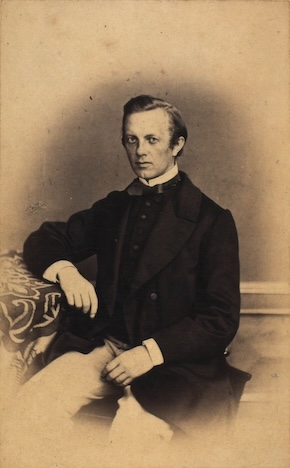
\includegraphics{heegaard.jpg}}
\hfill
\subfloat[Brandes]{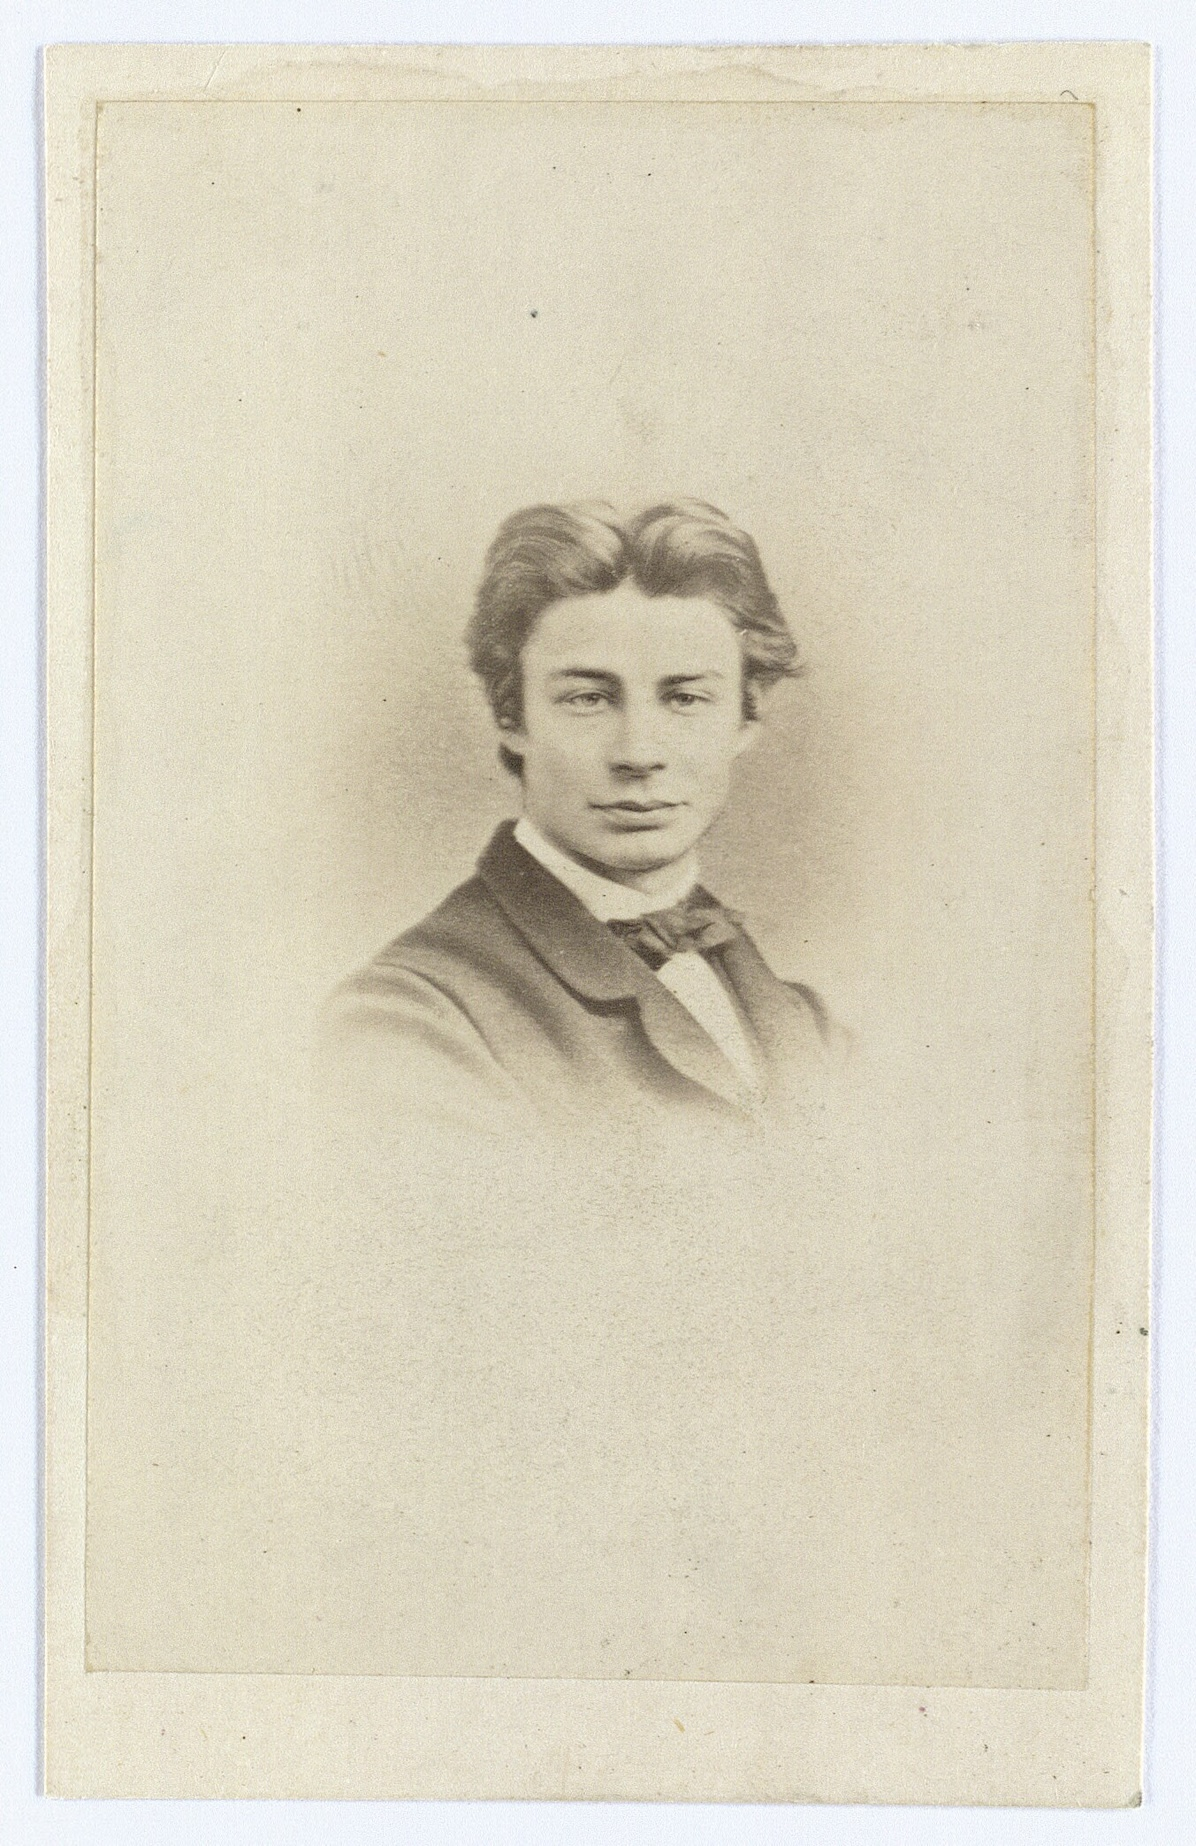
\includegraphics{brandes.jpg}}
\hfill
\subfloat[Høffding]{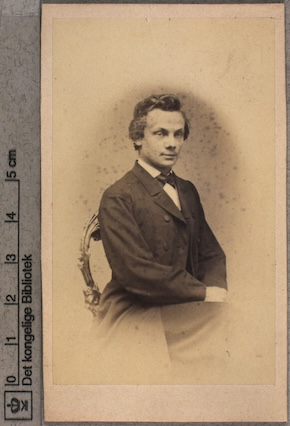
\includegraphics{høffding.jpg}}

\medskip
\subfloat[Kroman]{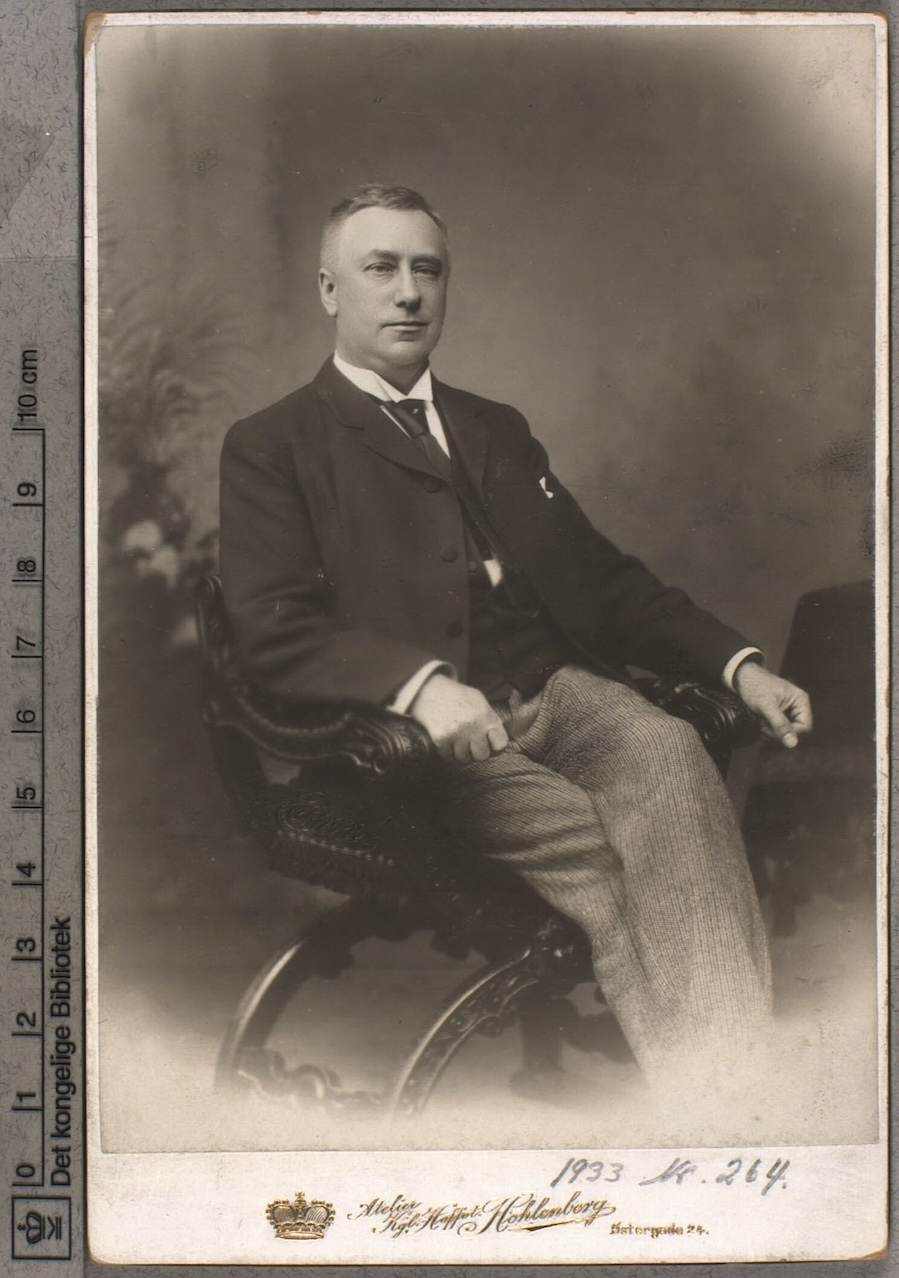
\includegraphics{kroman.jpg}}
\hfill
\subfloat[Ch. Bohr]{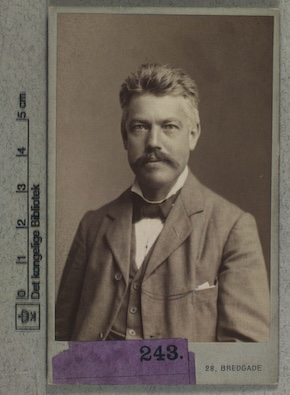
\includegraphics{christian.jpg}}
    \end{figure}

  
\end{frame}

\begin{frame}

\begin{figure}
  \centering 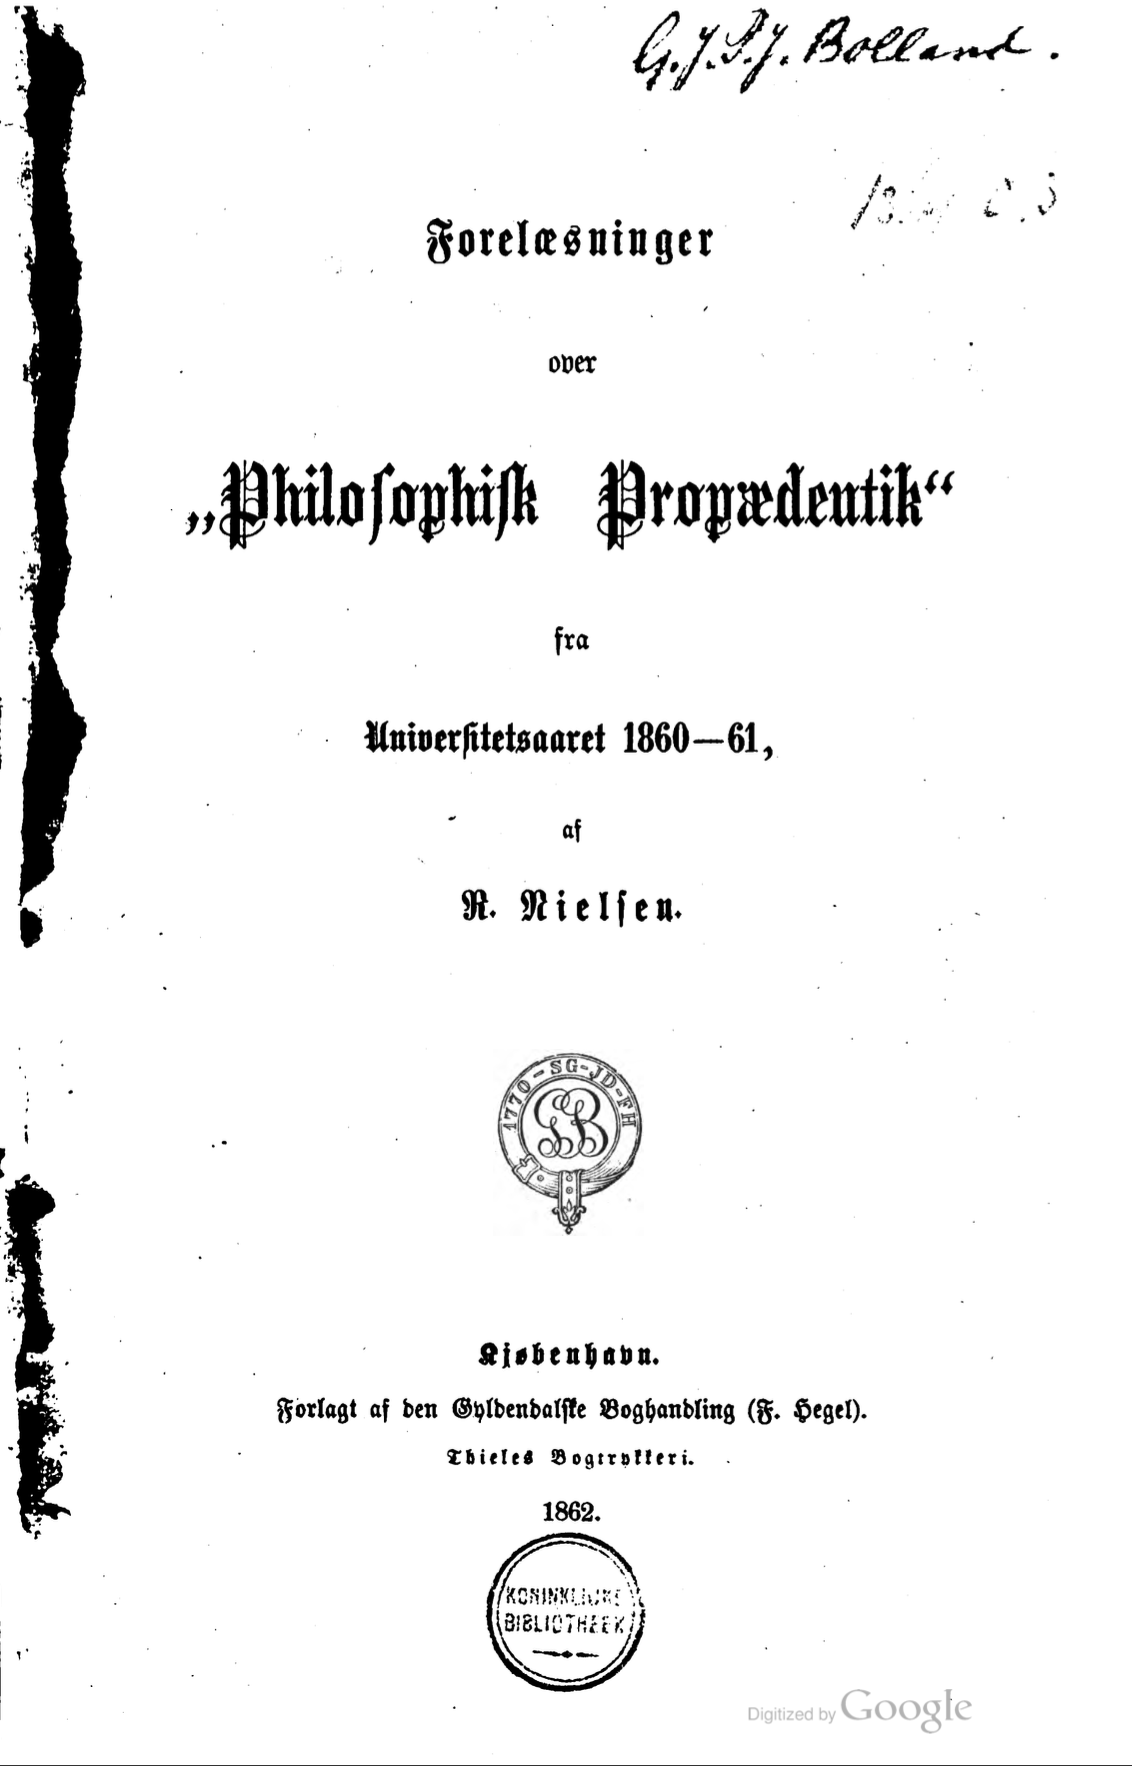
\includegraphics[scale=0.5]{prop1.png}
\end{figure}
\end{frame}

\begin{frame}

\begin{figure}
\centering
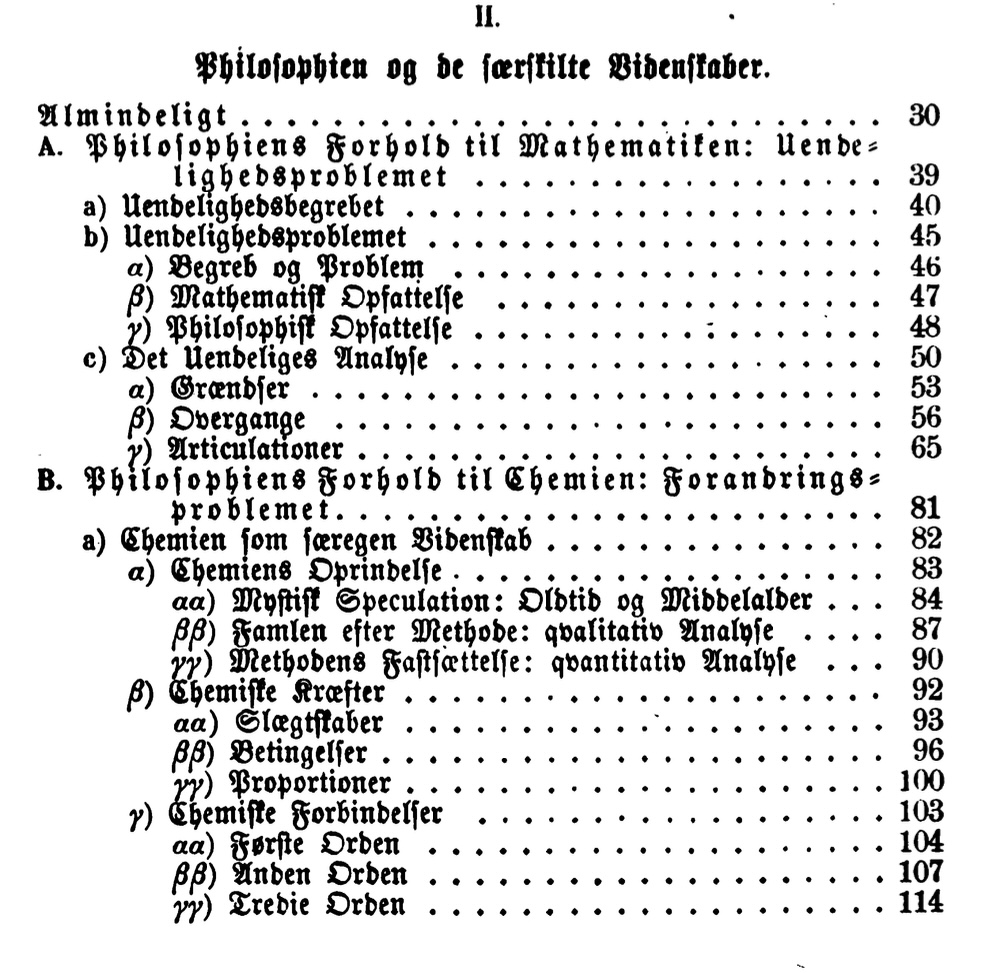
\includegraphics[scale=0.65]{prop2.jpg}
\end{figure}
\end{frame}

\begin{frame}

\begin{figure}
\centering
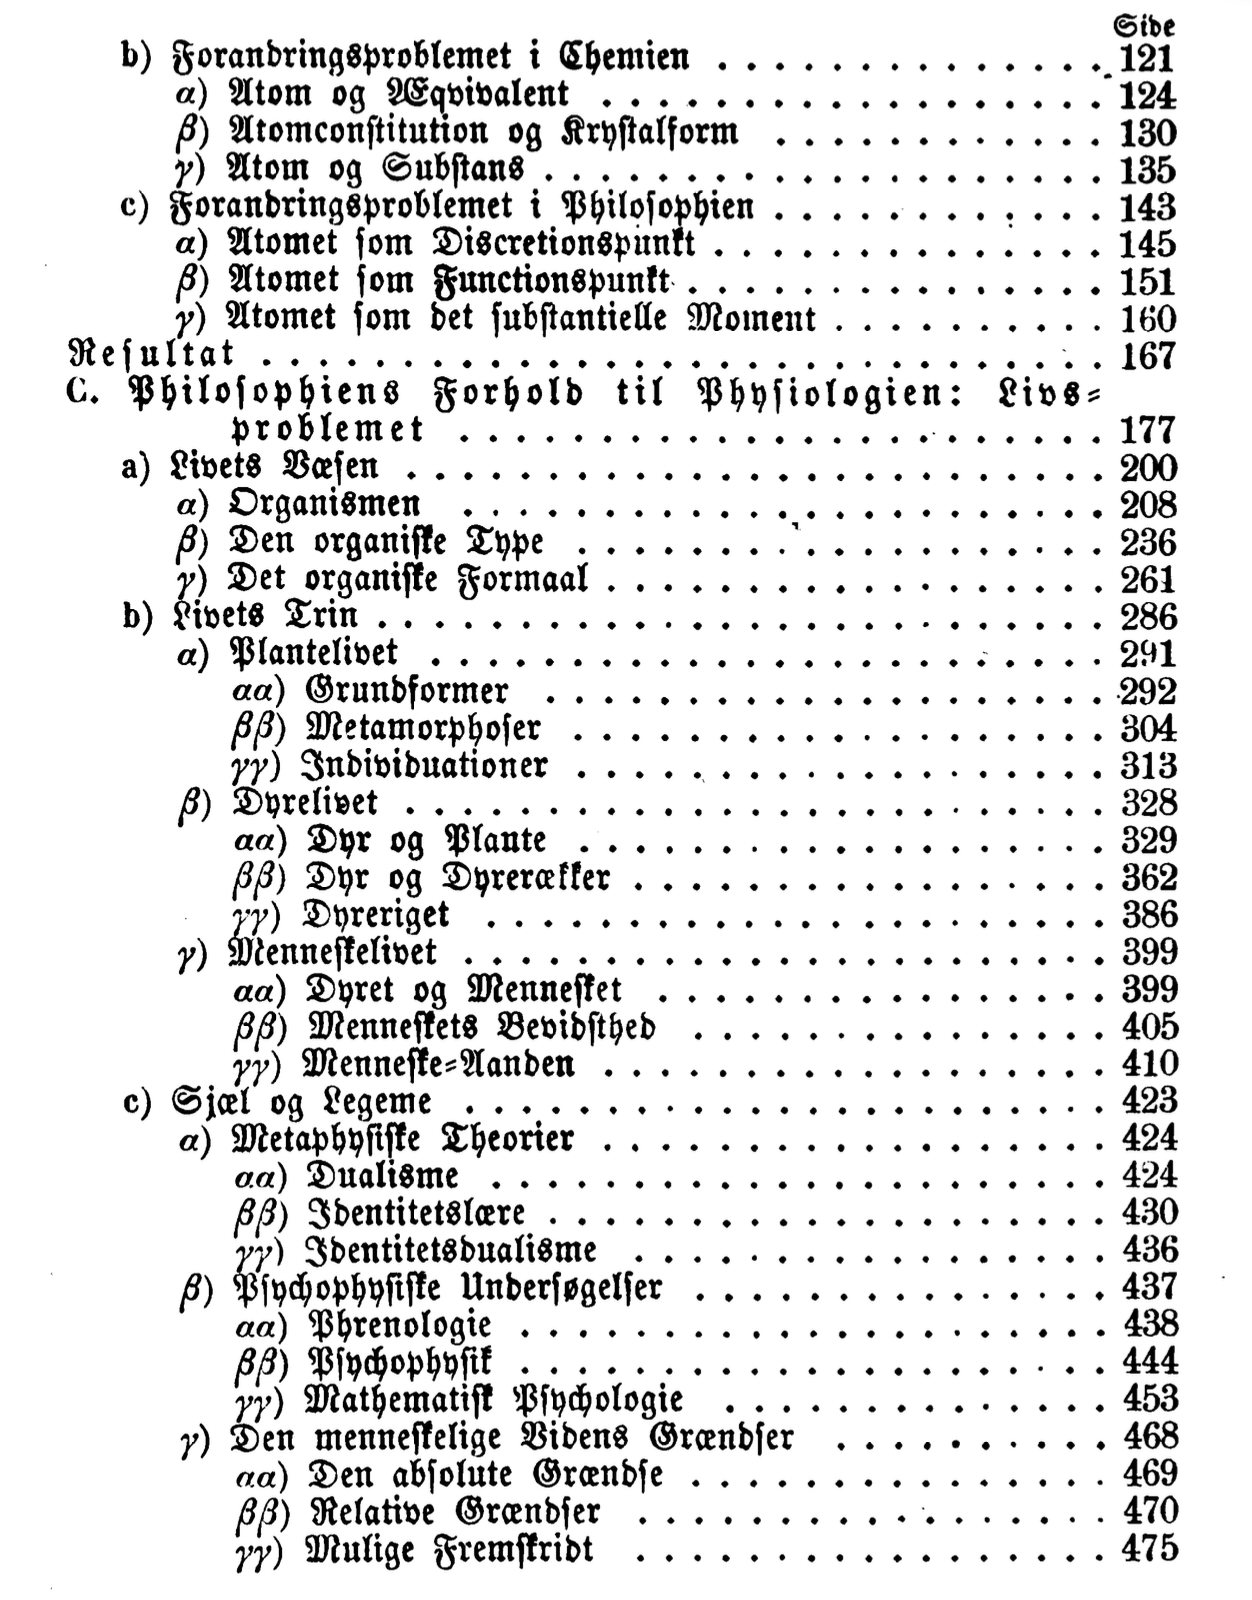
\includegraphics[scale=0.5]{prop3.jpg}

\end{figure}
\end{frame}

\begin{frame}

\begin{figure}
\centering
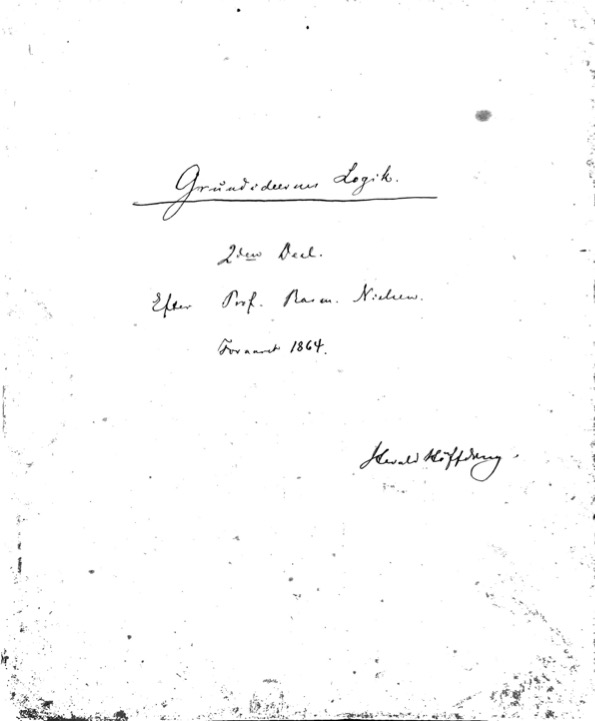
\includegraphics[scale=0.4]{høffding1.jpg}
\end{figure}

\end{frame}

\begin{frame}

\begin{figure}
\centering
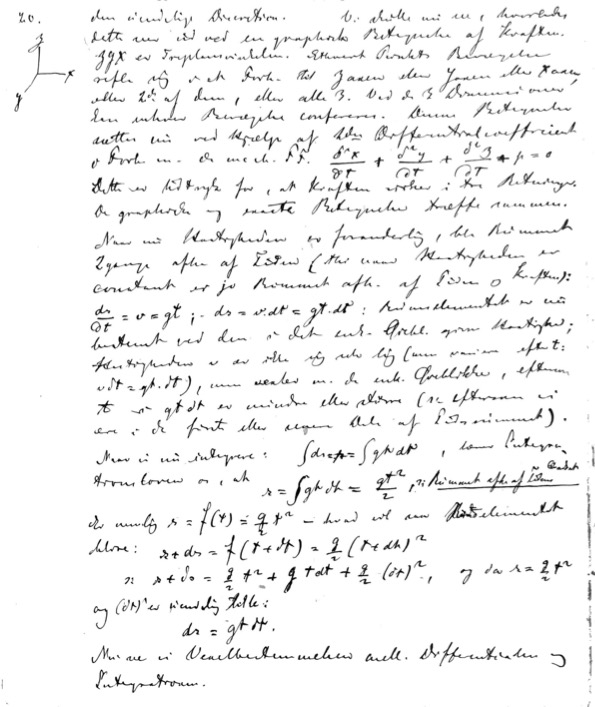
\includegraphics[scale=0.4]{høffding2.jpg}
\end{figure}
\end{frame}

\section{Subject and Object}

\begin{frame}{Hegel refresher}

\begin{itemize}
\item Elimination of distinction between subject and object (solution
  to post-kantian skepticism)
\item Elimination of distinction between reality (\emph{virkelighed})
  and concept (\emph{begreb})
  \begin{itemize}
  \item The real is the rational, and the rational is the real.
  \end{itemize}
\item Elimination of distinction between reason and cause
\item Insofar as science is rational, it is subsumed by philosophy.
\end{itemize}

\end{frame}

\begin{frame}{Kierkegaard's critique of (Hegelian) objectivity}

\begin{itemize}
\item No decision without subjectivity
\item A god's eye view description is unattainable for existing human
  beings
\end{itemize}
\end{frame}


\begin{frame}{Misunderstanding Bohr}

  \begin{itemize}
  \item Bohr talked about a moveable boundary (\emph{skillelinien})
    between subject and object.
  \item Contemporary physicists and philosophers misunderstand what
    Bohr was saying.
  \item For example, some think that Bohr was suggesting that the
    physicist draw a boundary between macroscopic and microscopic.
  \item John Bell called it Bohr's ``shifty split''.
  \item Many physicists and philosophers are busy trying to fix Bohr's
    ``confusion''.
  \end{itemize}


\end{frame}



\begin{frame}

  \begin{figure}
    \centering 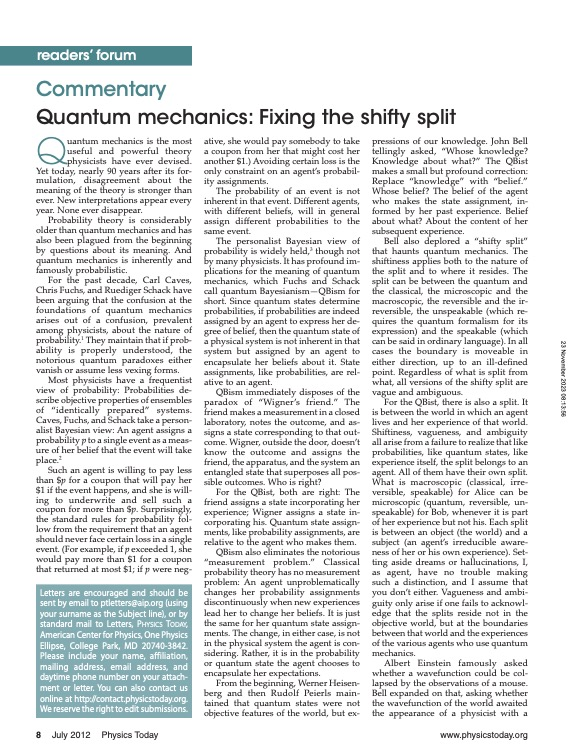
\includegraphics[scale=0.5]{mermin.jpg}
  \end{figure}

\end{frame}

\begin{frame}

  {\large \textbf{Hypothesis:} Bohr's talk about the movable line
    between subject and object is a continuation of the anti-Hegelian
    tradition of Poul Martin Møller, Søren Kierkegaard, and Rasmus
    Nielsen.}

  \bigskip {\large Bohr saw the utility of this idea for scientific
    practice, especially for attaining objective descriptions in
    situations where the subject is ``entangled'' with the object.}

\end{frame}

\begin{frame}

  \begin{quote}
    Every unambiguous communication about the state and activity of
    our mind implies of course a separation between the content of our
    consciousness and the background loosely referred to as
    ``ourselves'', but any attempt at exhaustive description of the
    richness of conscious life demands in various situations a
    different placing of the section between subject and
    object. \end{quote}

  \end{frame}
  \begin{frame}

    \begin{quote} In order to illustrate this important point, I shall
      quote a Danish poet and philosopher, Poul Martin Møller, who
      lived about a hundred years ago and left behind an unfinished
      novel called ``The Adventures of a Danish Student'', in which
      the author gives a remarkably vivid and suggestive account of
      the interplay between the various aspects of our position \dots
      (Bohr 1960, p 65)
  \end{quote}
\end{frame}

\begin{frame}

  \begin{itemize}
  \item Møller's novel gives a humorous description of a person
    (\emph{licentiaten}) who creates an endless series of new
    \emph{jeger}.
  \item The target of Møller's jest appears to be the Hegelian
    aspiration to achieve objectivity through infinite reflection.
  \item Møller never states clearly his objections, or his alternative
    vision.
  \item SK makes the objection more forcefully.
  \item But SK doesn't leave us with any suggestions about the
    positive role of \emph{viden} or \emph{videnskab}.
  \end{itemize}

\end{frame}

\begin{frame}

\begin{figure}
  \centering 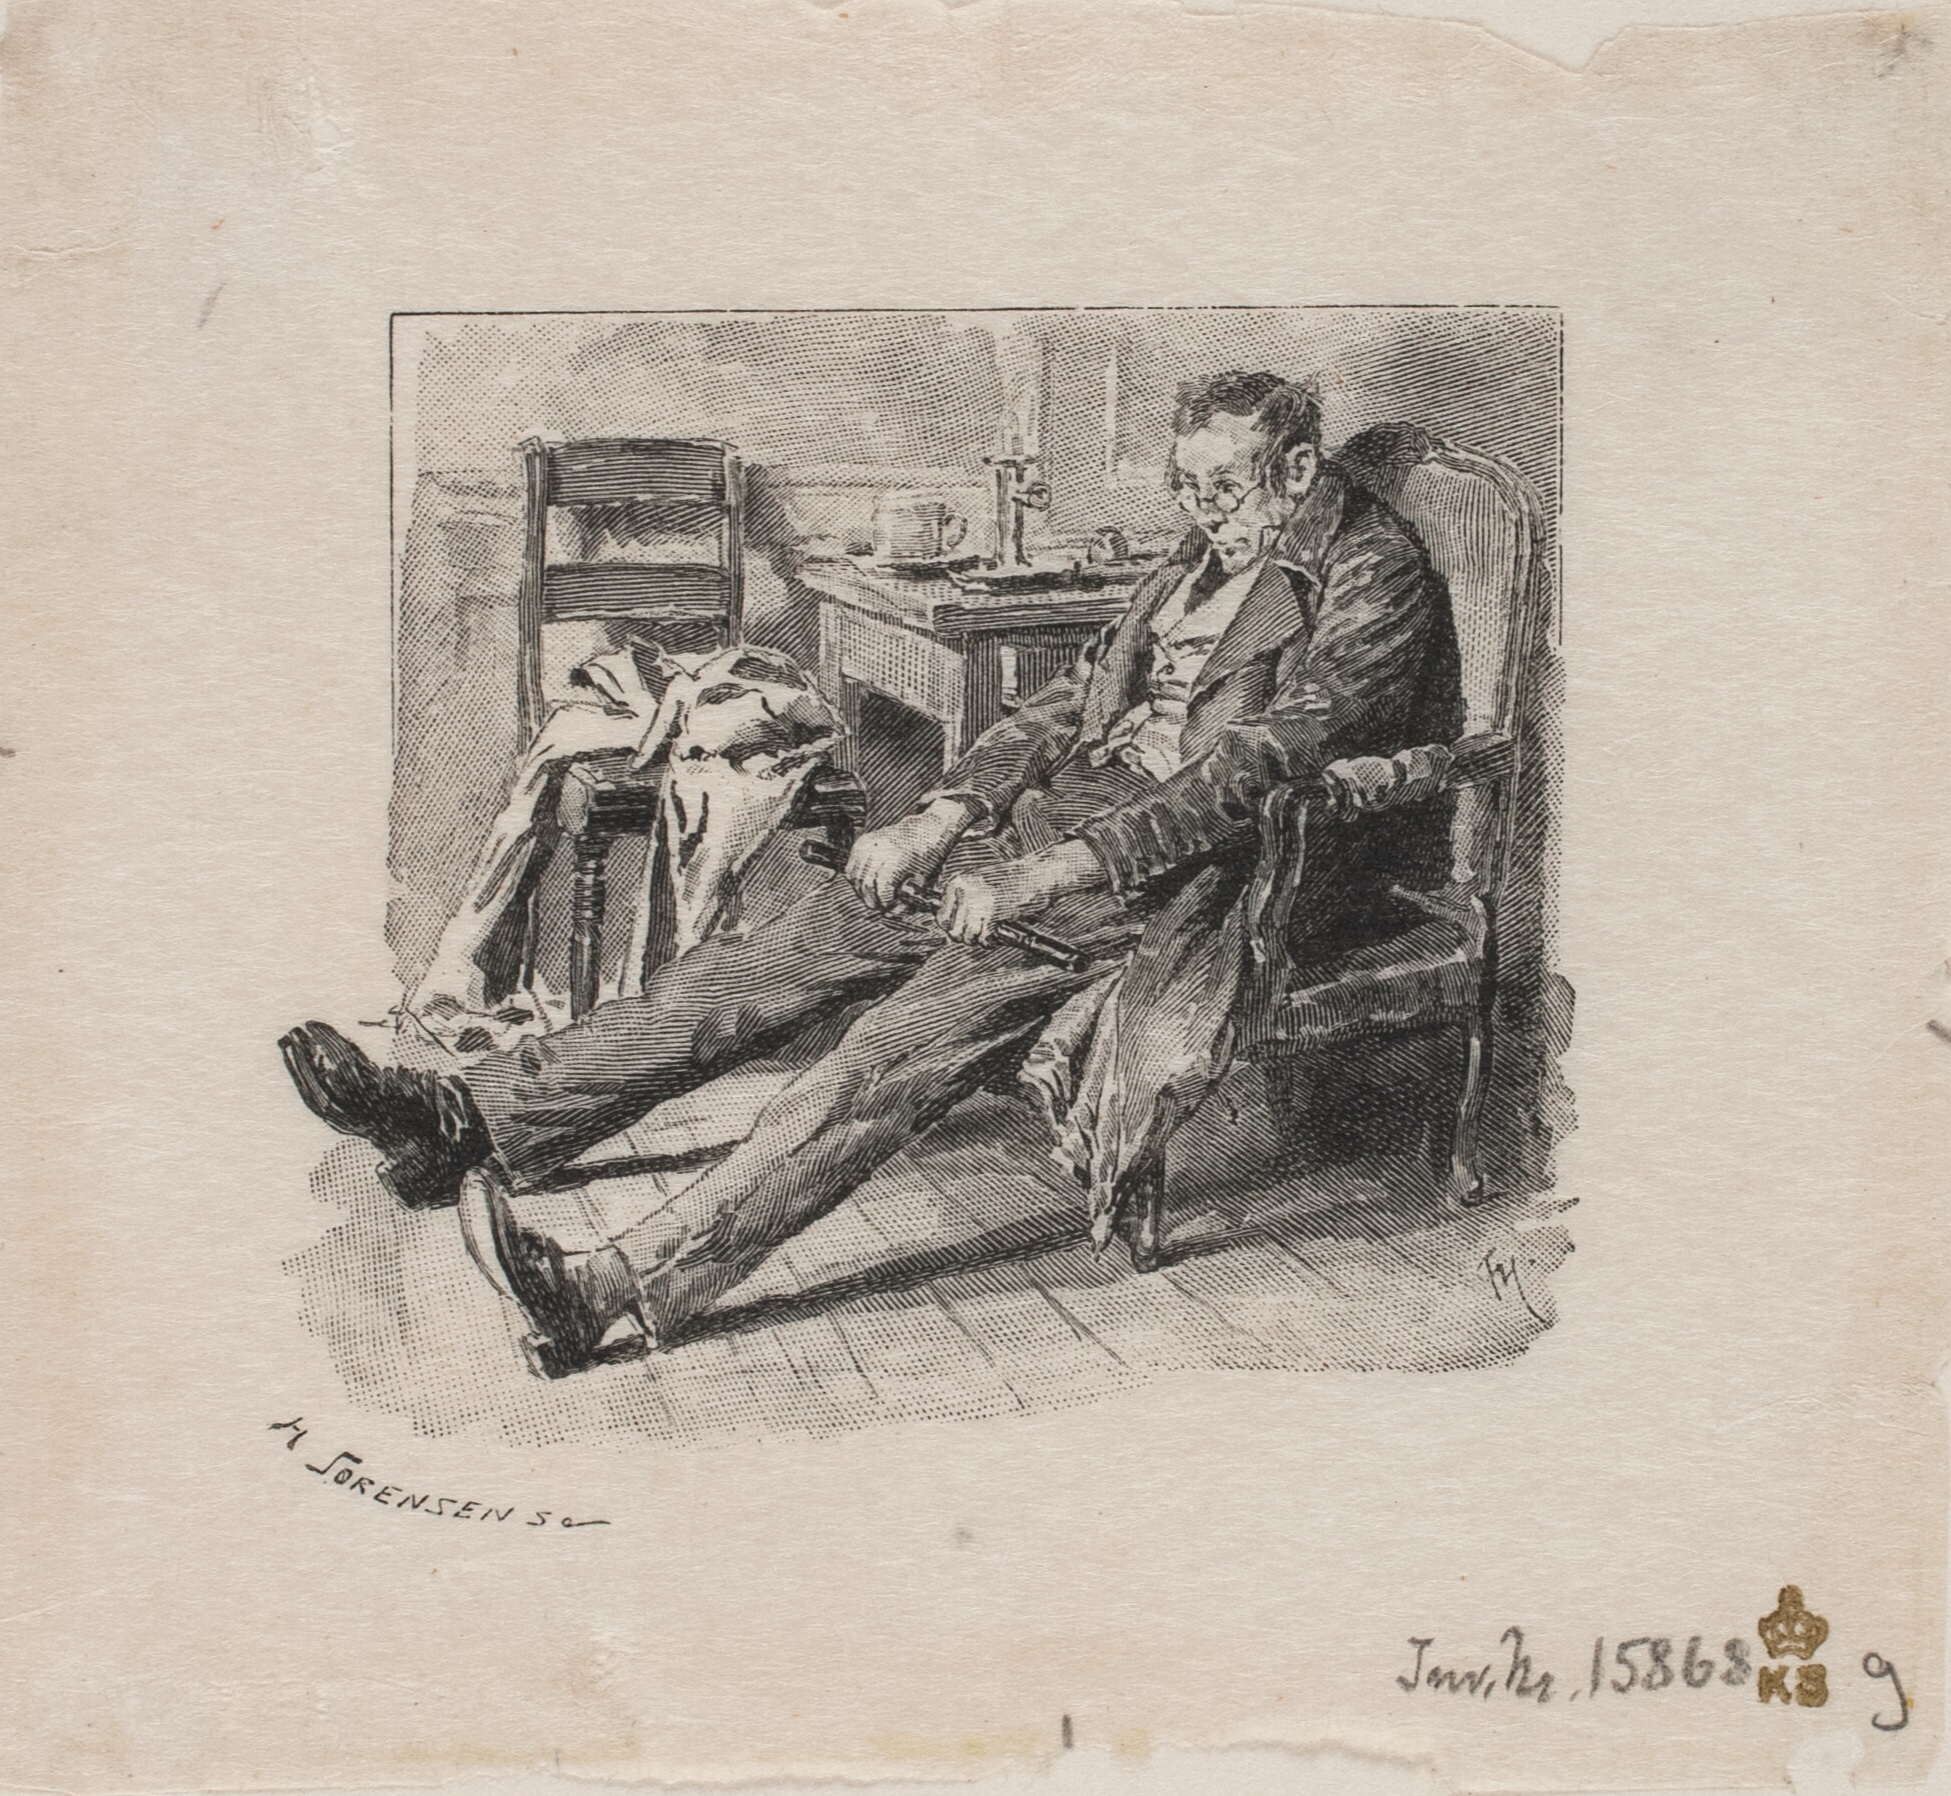
\includegraphics[scale=0.1]{licentiate.jpg}
\end{figure}
\end{frame}

\begin{frame}

  \begin{quote}
    Actually, ordinary language, by its use of such words as thoughts
    and sentiments, admits typical complementary relation between
    conscious experiences implying a different placing of the section
    line between the observing subject and the object on which
    attention is focussed. We are here presented with a close analogy
    to the relationship between atomic phenomena appearing under
    different experimental conditions and described by different
    physical concepts, according to the role played by the measuring
    instruments. \end{quote} \end{frame}

\begin{frame}

  \begin{quote} In fact, the varying separation line between subject
    and object, characteristic of different conscious experiences, is
    the clue to the consistent logical use of such contrasting notions
    as will, conscience and aspirations, each referring to equally
    important aspects of the human personality. (Bohr 1953, pp
    389-390)
\end{quote}
\end{frame}

\begin{frame}

\begin{quote}
  In emphasizing the necessity of paying proper attention to the plac-
  ing of the object-subject separation in unambiguous communication,
  the modern development of science has created a new basis for the
  use of such words as knowledge and belief. (Bohr 1955, p 61)
\end{quote}
\end{frame}


\begin{frame}


  \begin{itemize}
  \item As already mentioned, the large majority of contemporary
    thinkers don't see anything interesting in Bohr's talk about
    subject and object.
  \item Favrholdt thought that Bohr received inspiration from reading
    Poul Martin Møller, but otherwise he created these great new ideas
    completely from scratch.
    \begin{itemize}
    \item He unequivocally denies any influence by
      Kierkegaard. \end{itemize}
  \end{itemize}


\end{frame}

\begin{frame}

  {\large \textbf{Hypothesis:} Nielsen inherits the idea of the
    moveable boundary from Møller and Kierkegaard, and he sharpens it
    into a form that is applicable in philosophy of science.}

  \bigskip {\large \textbf{Corollary:} Kierkegaard influences science
    (including Bohr's approach to quantum physics) via Nielsen.}

\end{frame}

\begin{frame}

  Nielsen: The boundary between apriori and aposteriori is moveable.

  \medskip \begin{quote} But when the boundary between apriori and
    empirical is supposed to be conceived of as definite and exact,
    then troubles arise. (1880, p 30)
\end{quote}

\medskip \begin{quote}
  A fixed, unmovable boundary line between the apriori and aposteriori
  cannot be set. (1880, p 37)
\end{quote}
\end{frame}

\begin{frame}

  \textbf{Objectiveringslov}

  \medskip \begin{quote} No Object without a corresponding
    Objectification; it is an a priori law that underwrites all
    empiricism, a basic law that in science is, if possible, even more
    unshakable than Newton's law of gravity. From this it can be seen,
    that a critical boundary, a boundary line, on whose one side we
    have the objectivizing subjectivity, while the object is standing
    on the other side, is confusing and meaningless. (1880, p 41)
\end{quote}
\end{frame}

\begin{frame}{Rosenberg on Nielsen}

  \begin{quote} Her fremsætter Nielsen den 'Objektiveringslov', som
    senere blev et saa betydningsfuldt Led i hans Metafysik:
    Objekterne kan ikke objektivere sig selv, og da Objekter uden
    Objektivering er umulige, forudsætter Objektiviteten en
    objektiverende Subjektivitet. Paa den anden Side kan
    Subjektiviteten ikke undvære Objektiviteten, eftersom dens
    Selvbegriben og Selvmagt saa vilde blive uden Indhold.
\end{quote}

\end{frame}

\begin{frame}{Rosenberg on Nielsen}

  \begin{quote}
    Opfatter vi Forholdet udialektisk faar vi en kritisk Adskillelse
    som hos Kant, der ganske fornagler Problemet om Subjektets og
    Objektets indbyrdes Forhold, eller en mystisk Realisme som hos
    Schelling, der fortoner Problemet i Taage.  Men naar
    Objektiviteten og den bærende Subjektivitet paa ethvert Punkt
    dialektisk ses at forudsætte hianden, da forstaas `Naturens
    aandrige Aandløshed', og man øjner Muligheden af Problemets
    Løsning --- saavidt muligt er paa menneskelige Vilkaar. (Rosenberg
    p 13) \end{quote} \end{frame}

\begin{frame}{Høffding on Nielsen}
  
  \begin{quote} Nielsen imagined that to describe the
    interrelationship between the subjective and the objective, or as
    he calls it, knowledge and power, an infinite analysis would be
    needed, since every subject presupposes an object, and every
    object in turn a subject. When one does not want to conclude in a
    speculative and theological way, it becomes a duel
    [\emph{Holmgang}] without end.
  \end{quote}
  
\end{frame}

\begin{frame}

  \begin{quote}
    \ldots Nielsen did not perceive the matter in this way. His way of
    thinking was that since every object must be objectified,
    i.e.~presupposes a subject, and since the human subject cannot
    perceive (objectify) everything, there must, if the reality of
    objects is to be asserted, be an absolute (`ontological') subject
    for whom the absolute reality exists.
\end{quote}

\end{frame}

\begin{frame}

  \begin{quote}
    He overlooks the fact that the game must begin again here; even a
    God would be bound to the Law of the Relation between Subject and
    Subject and Object. The attempt to justify an abstract theism
    through \emph{Grundideernes Logik} has therefore not succeeded. We
    could not get further than to determine and describe a subject in
    relation to which certain phenomena (objects) apply, just as the
    astronomer must determine a point (on the earth, on the sun, or
    wherever) from which the positions and movements of the celestial
    bodies could be described as if they were absolute. (Høffding
    1909, p 189-190)
\end{quote}

\end{frame}


\begin{frame}{Was Rasmus Nielsen the first analytic philosopher?}

\begin{itemize}
\item circa 1900: Bertrand Russell and G.E. Moore reject Cambridge
  Hegelianism
\item circa 1915: Wittgenstein reads Kierkegaard
  \begin{itemize}
  \item ``language on holiday''
  \item ``logic must take care of itself''
  \end{itemize}
\item
  The logical positivists argue that philosophy has no content of its
  own; instead, it is to be the logic of science
\end{itemize}
\end{frame}

\section{Conclusion}

\begin{frame}{Open questions: backward}
\begin{itemize}
\item Low-hanging fruit in research on 19th century Danish
  philosophers

  \begin{itemize}
  \item Reading and interpreting Nielsen's books is a big job: Danish,
    fraktur, mathematics, etc.
  \item Nielsen's handwritten papers in KB
  \item Notes by students in KB
  \end{itemize}
\item Can we say something more specific about what triggered
  Nielsen's turn to \emph{fagvidenskaberne}?

  \begin{itemize}
  \item The timeline between 1853 and 1860 is a bit hazy
  \end{itemize}
\end{itemize}
\end{frame}

\begin{frame}{Open questions: backward}

\begin{itemize}
\item What role does the concept of power (\emph{Magt}) play for
  Martensen and Nielsen?
\item The notion of \emph{objectivering} does heavy lifting for
  Nielsen, and it appears already in \emph{Den Propædeutiske Logik}
  (1845). Does it appear elsewhere before that? Do other Danish
  philosophers use the concept?
\item Did Nielsen know about non-euclidean geometry, and did that
  influence his view about the moveable apriori?
\end{itemize}
\end{frame}

\begin{frame}{Open questions: forward}

\begin{itemize}
\item Does RN represent a betrayal of SK's ideas, or an innovative
  application of these ideas to a life with more typically modern
  concerns?
\item
  Does RN provide a positive development of SK's conception of the role
  of objective knowledge in a good human life?
  \begin{itemize}
  \item Does Nielsen provide an alternative to the views of Spinoza
    and Hegel?
  \end{itemize}
\item Does RN have any helpful ideas about the relationship between
  science, philosophy, and theology?
\end{itemize}
\end{frame}

\begin{frame}{Further reading}

  \begin{itemize}
  \item Stewart. ``Rasmus Nielsen: From the object of `prodigious
    concern' to a `windbag'\,''
  \item Garff. \textit{Søren Kierkegaard: A Biography}
  \item Koch. \emph{Den Danske Idealisme} (chapter on
    Nielsen)
  \item Høffding. \emph{Danske Filosoffer} (chapter on Nielsen)
  \item For primary sources, I recommend Nielsen's late works
    \textit{Almindelig Videnskabslære i Grundtræk} and
    \textit{Philosophiske Grundproblemer}
  \end{itemize}

\end{frame}

\end{document}

%%% Local Variables:
%%% mode: latex
%%% TeX-master: t
%%% End:

\begin{frame}{Empiricism}

\begin{itemize}
\item
  Both by example and in word, Nielsen supported the empirical sciences
\item The anti-logical
\end{itemize}
\end{frame}

\begin{frame}{Objectivity}

Nielsen rejects the Hegelian aspiration for presupposition-free
knowledge

\begin{quote}
From subjective presuppositions proceed objective consequences, and from
objective consequences, objective knowledge. (1880, p 44-45)
\end{quote}
\end{frame}


\begin{frame}{Nielsen's Theistic Logic Program}

  Nielsen: Only Theism prevents collapse to idealism or dogmatism

  \medskip \begin{quote} Saalænge Forholdet imellem den reflecterende
    Subjectvitet og den objective Verden eensidig fastholdes under
    Endelighedens Synspunkt, vil al vor Begriben og Erkjendelse idelig
    vakle imellem a) en kritisk Idealisme paa den ene og b) en mystisk
    Realisme paa den anden Side.  (1845, p 205)
  \end{quote}

\end{frame}



\begin{frame}{Viden og Magt}

\begin{itemize}
\item Even in his early work, Nielsen argued that creation was an act
  of will (demonstration of power) by God
\end{itemize}

A being with complete knowledge must also have complete power.

\begin{quote}
If there is a complete knowledge, then it cannot be sensory; it must get
a grip on the realities in a completely unique way, namely by the fact
that it originally brings them forth. (1880, p 60)
\end{quote}

\end{frame}

\begin{frame}{Mechanism versus Vitalism}

  Nielsen denies the existence of a special life substance

  \medskip
  \begin{quote}
  A scientifically conducted physiology must necessarily lead to the
  result that there is no ``life force'' distinct from nature's
  ordinary forces. (1862, p 187)
\end{quote}

\end{frame}

\begin{frame} Methodological naturalism

\begin{quote}
  The deeper science penetrates into some state of affairs, all the
  more clear it becomes that these challenges in their parts as on the
  whole, in the smallest as in the largest, are solved in a natural
  way and by natural means. (1862, p 187)
\end{quote}
\end{frame}

\begin{frame}{Faith and Reason}

\begin{itemize}
\item Nielsen refers to Darwin's \emph{Origin of Species} in his 1861
  lectures --- the first reference in the Danish literature
\item ``Et synspunkt for Darwinisme'' (1873). Nielsen argues that
  accepting Darwinian evolution is fully consistent with Christian
  doctrines of creation, fall, etc.
\end{itemize}
\end{frame}

\begin{frame}{Philosophy of Science}
  Nielsen rejects the idea of a single absolute science.

\begin{quote}
  What Schelling calls ``science itself'' cannot possibly survive
  ``the sciences'' (1880, p 72)
\end{quote}

\begin{quote}
  That each distinct science must have its distinct starting point,
  conditional upon substance on topic, follows from the nature of the
  matter. (1880, p 89)
\end{quote}
\end{frame}
